This section details the usage of individual calorimeter towers for EMCal, inner and outer HCal. 

\subsection{Tower Energy Reconstruction}
\label{sec:towerenergyreco}

Our analysis used the central production of calorimeter data in which waveforms above a set software zero suppression level are processed using the TEMPLATE mode of the CaloWaveformProcessing module. 
For Run 2024, tower-by-tower hardware zero suppression (ZS) thresholds were implemented to reduce data volume. 
Calorimeter tower waveforms with recorded pre-minus-post values below the ZS threshold only recorded the pre and post samples of the waveform and pre-minus-post values above the ZS threshold recorded the full 12 time sample waveform. 
During the fitting step of the calorimeter tower reconstruction, an additional software level ZS threshold is applied to correct for biases in the calorimeter energy distribution from noise waveforms. 
This ZS threshold is higher than the hardware level threshold and uniform across the full detector; for calorimeter tower waveforms which fall below this software level ZS threshold, the pre and post sample values of the waveform are used instead of fitting the waveform using the template fit method. 
For this anaylsis, the software level ZS thresholds were set to 100 ADC for the EMCal and 50 ADC for each of the HCals.

Both EMCal and HCal templates were created using beam data from early runs of Run 2024. 
The template fit has three free parameters: the pedestal, peak time and scale of the waveform, and the processing procedure returns these parameters plus a $\chi^{2}$ term which acts as a goodness of fit metric. 
More information on the template fit method can be found in the EMCal Year1 Calibration Note \cite{Seidlitz1}.

All three calorimeters, EMCal, IHCal and OHCal, are calibrated to the electromagnetic energy scale. 
For the EMCal, an $\eta$ dependent $\pi^{0}$ calibration is established using a subset of good beam runs. 
The run group specific calibration used for this analysis is measured using beam data from runs 54909 to 54920. 
More information regarding the specifics of the EMCal calibration can be found in the EMCal Year1 Calibration Note \cite{Seidlitz1}. 
The IHCal and OHCal are both calibrated to the EM energy scale using the minimum ionizing particle energy depositions from cosmic ray muons. 
The cosmics data used for this analysis's IHCal cosmics calibration were taken in a 30 day period that spans both before and after the beam run period used for this analysis and the cosmics data used for this analysis's OHCal cosmics calibration where taken in a 5 day span directly after the beam run period used for this analysis. 
Therefore, it is expected that the detector conditions are fairly consistent between cosmics and beam running and any detector condition effects should be accounted for in the calibration from cosmics data. 
An additional HCal calibration step of a tower-slope correction is applied to account for inconsistencies in the cosmic data simulation; here a relative calibration is applied to HCal towers using the assumptions of $\phi$ symmetry and that the absolute cosmics-based calibrations of the HCal towers on the sides of the detectors with very high statistics are accurate.

An additional calibration was applied to the ZS tower energies to account for the ZS algorithm, waveform sample 6 - sample 0, underestimating the tower energy.
The calorimeters on the whole are timed in at sample 6, however for multiple reasons including differences in trigger latching time samples, intra-sector cable lengths and tower distances to the collision points, on the tower–by-tower level, a tower may not be timed in exactly at sample 6.
While the template fit has little to no constraints within the waveform length on the signal timing when looking for the signal peak, the ZS algorithm expects the signal peak to be timed in exactly at sample 6. 
Therefore, a cross calibration is applied to the zero suppressed waveforms to account for shifts in the tower-by-tower mean time of signal peaks. 
This ZS cross calibration is determined using the ratio of $\frac{\overline{ADC}_{\text{Template fit}}}{\overline{ADC}_{\text{ZS}}}$ for well defined signals, signals with $ADC_{\text{Template fit}}$ = [200,2000] ADC for EMCal and $ADC_{\text{Template fit}}$ = [100,2000] ADC for HCals, extracted from the calorimeter fitting step of the calorimeter data production chain using the CaloFittingQA module. 
These cross calibration factors are determined on a tower-by-tower and run-by-run basis to account for tower-by-tower timing differences. 

Additionally, cross checks for the calorimeter sampling fraction has been performed to verify the response of the individual calorimeter towers and its $\eta$ dependence. 
It was determined that for this analysis, the uniform sampling fraction included in the G4\_HcalIn\_ref and G4\_HcalOut\_ref macros, which were determined from simulation particle gun studies, can be used, since the HCal absolute energy scale calibration is determined on the scintillator EM energy level and the same sampling fraction was applied to both simulation and data. 
Therefore, this sampling fraction value applied in both data and MC cancels out in the correction step when extracting measurements of the truth level \detdeta. 
%These studies are detailed in Appendix~\ref{sec:SamplingFrac}. 
Furthermore, during analyzing the data, the effect of implementing the realistic support structure into the simulation software package was found to be crucial. 
%The detailed studies of the impact of the support structures for this analysis can be found in Appendix.~\ref{sec:support_structure}.

\subsection{Vertex Dependent $\eta$ Correction}
The transverse energy per pseudorapidity unit, \detdeta, is calculated in a given $\eta$ interval based on the $\eta$ position of individual calorimeter towers in the lab frame.
To take into account the position of the collision vertex, the $\eta$ value in each tower is corrected event-by-event relative to the vertex position of the collision. 
In the runs used for this analysis, x \& y vertex reconstruction was not possible due to absent of tracker detector data, and therefore only a correction for the z-coordinate is obtained. In simulation and data, a corrected tower $\eta$ is calculated for each tower as
\begin{equation}
    \eta_{\text{corrected}} = \sinh^{-1}\left(\frac{z_{\text{new}}}{\sqrt{x^2_{\text{new}}+y^2_{\text{new}}}}\right),
\end{equation}
where
\begin{gather}
    x_{\text{new}} = x_{\text{tower}} - x_{\text{vertex}}
    \\
    y_{\text{new}} = y_{\text{tower}} - y_{\text{vertex}}
    \\
    z_{\text{new}} = z_{\text{tower}} - z_{\text{vertex}},
\end{gather}

and $x_{\text{tower}}$, $y_{\text{tower}}$, \& $z_{\text{tower}}$ are the $x$, $y$, \& $z$ positions of the towers with respect to the center of the detector. $x_{\text{vertex}}$, $y_{\text{vertex}}$, \& $z_{\text{vertex}}$ are the $x$, $y$, \& $z$ positions of the vertex. 
In data and simulation, $z_{\text{vertex}}$ is determined by reconstruction via the MBD.

With no $x$ or $y$ correction due to the lack of $x$ or $y$ vertex determination, this reduces to

\begin{equation}
    \eta_{\text{corrected}} = \sinh^{-1}\left(\frac{z_{\text{new}}}{\sqrt{x^2_{\text{tower}}+y^2_{\text{tower}}}}\right) = \sinh^{-1}\left(\frac{z_{\text{new}}}{r_{detector}}\right),
\end{equation}

with $r_{detector}$ the radius of the detector subsystem in question (EMCal, IHCal, or OHCal).  
The uncertainty in our event-by-event $\eta$ calculation due to no $x$ or $y$ vertex determination was found to be negligible for all calorimeters for $x$ or $y$ vertex shifts of up to 2 cm well beyond the nominal x and y vertex width of 0.01 cm.
A schematic of this event by event $\eta$ correction is given in Fig. \ref{fig:eta_determination}.

\begin{figure}
    \centering
    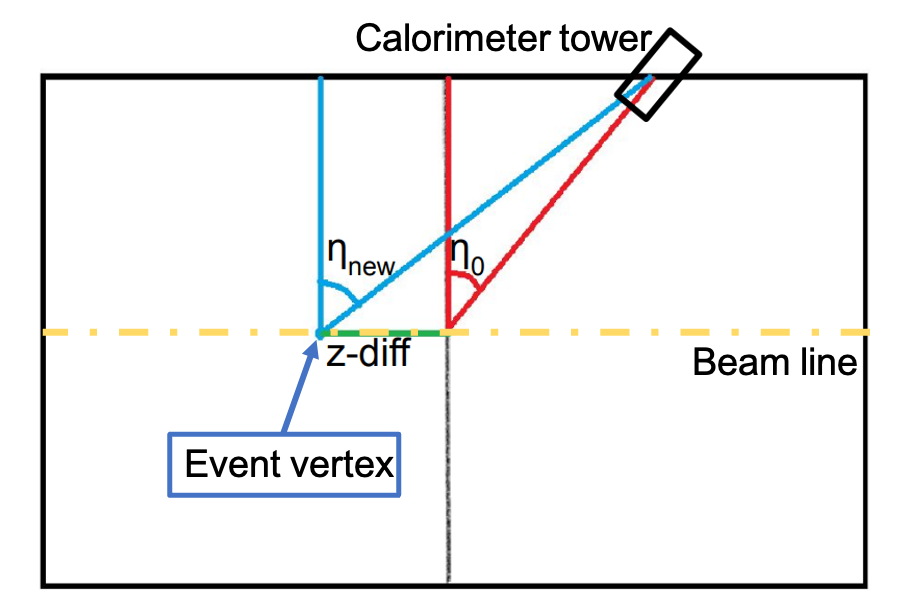
\includegraphics[width=0.7\linewidth]{detdeta/Figures/zvertex_reweighting/eta_determination.png}
    \caption{Event by event determination of calorimeter tower $\eta$ based on the z vertex of the event.}
    \label{fig:eta_determination}
\end{figure}

These new $\eta$ values are used as the values for determining $\ET$ as

\begin{equation}
    \ET = \frac{E_{\text{tower}}}{\cosh\eta_{\text{corrected}}}.
\end{equation}

$E_{\text{tower}}$ is the energy deposited in a given tower in data or simulation.

\subsection{Uncorrected \& Reconstructed Simulated \detdeta}
To obtain uncorrected (reconstructed from data) or reconstructed simulated \detdeta for a given run and centrality class, $\ET$ is first calculated for each calorimeter tower as
\begin{equation}
    E_{\text{T,tower}}=E_{\text{tower}}/\cosh\eta
\end{equation}
this value is corrected for bin width and used to fill a 1-D TProfile in $\eta$. 
This TProfile is then converted to a histogram to scale each of the bins in $\eta$ by their respective bin widths. In total, we create 5 histograms of the reconstructed \detdeta, a reconstructed \detdeta from each of the individual calorimeters using only contributions from that calorimeters' towers (e.g. the EMCal \detdeta measurement only has contributions from EMCal towers), a HCal reconstructed \detdeta histogram comprising both layers of the HCal, and a full calorimeter reconstructed \detdeta histogram which is filled with tower contribution from all three calorimeters. 
Our reconstructed full calorimeter measurement is the same as the sum of the reconstructed individual calorimeter measurements; there is no additional weighting applied on our part between contributions of the hadronic calorimeters versus EM calorimeter applied to our full calorimeter reconstructed \detdeta. 
Additionally, the detector acceptance determined from hot tower masking in data is applied identically to both data and simulation, ensuring the reconstruction level \detdeta in both data and simulation is determined from the same detector acceptance. 
Fig.~\ref{fig:dEtdeta_reco} shows the detector-level \detdeta measurements for all calorimeter layers for both data and simulation samples for the 0-5\% most central events; reconstructed \detdeta measurements for all centrality bins are included in Appendix~\ref{sec:full_detdeta_plots}.

\begin{figure}
    \centering
    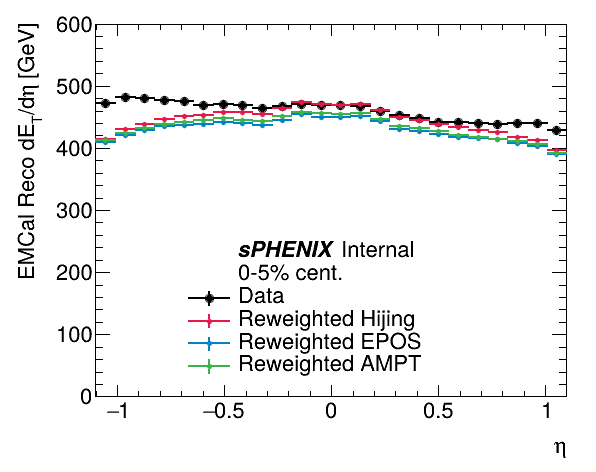
\includegraphics[width=0.48\linewidth]{detdeta/Figures/dETdeta_measurements/emcal_reco_0-5.png}
    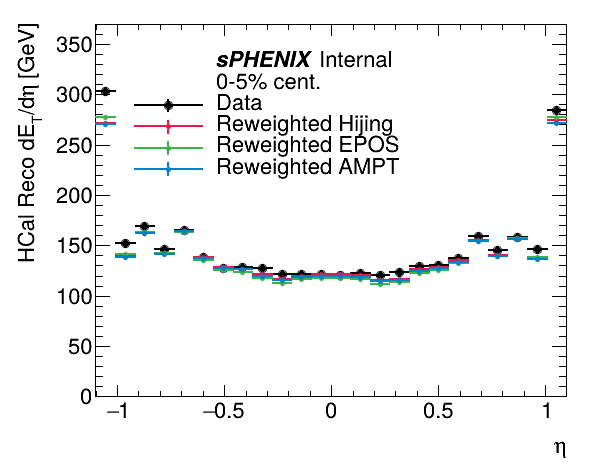
\includegraphics[width=0.48\linewidth]{detdeta/Figures/dETdeta_measurements/hcal_reco_0-5.png}
    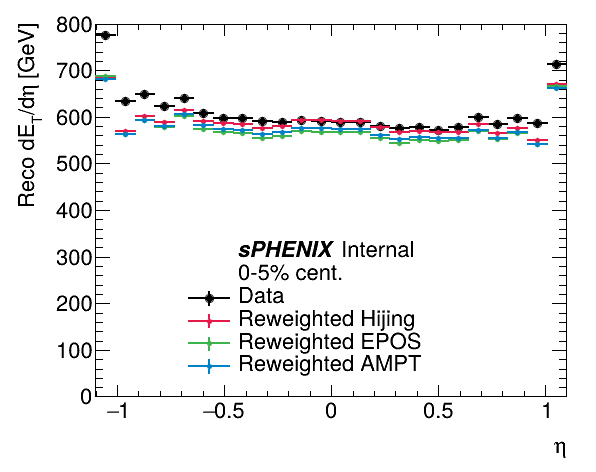
\includegraphics[width=0.48\linewidth]{detdeta/Figures/dETdeta_measurements/calo_reco_0-5.png}
    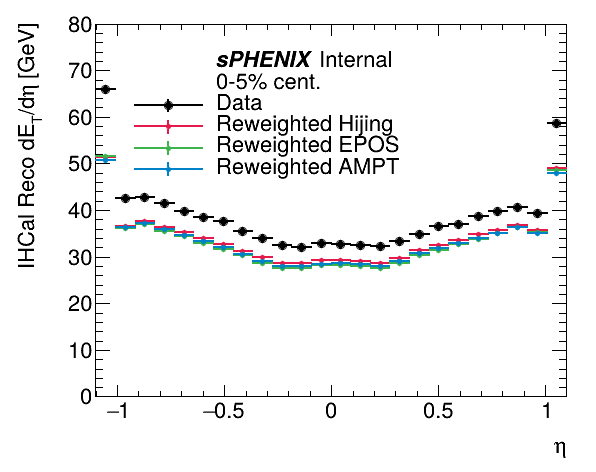
\includegraphics[width=0.48\linewidth]{detdeta/Figures/dETdeta_measurements/ihcal_reco_0-5.png}
    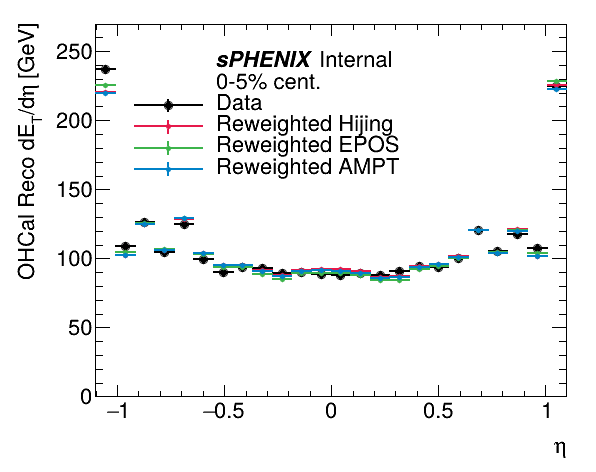
\includegraphics[width=0.48\linewidth]{detdeta/Figures/dETdeta_measurements/ohcal_reco_0-5.png}
    \caption{Reconstructed \detdeta for 0-5\% central events for EMCal (top left), HCal (top right), Full Calorimeter (middle left), IHCal-only (middle right), and OHCal-only (bottom), compared to the reconstructed \detdeta from simulated events of reweighted EPOS, AMPT and HIJING.}
    \label{fig:dEtdeta_reco}
\end{figure}

\subsection{Truth \detdeta}
Truth \detdeta is calculated by binning $E_{\text{T,particle}}=E_{\text{particle}}/\cosh\eta$ in a 1-D histogram over $\eta$ after correcting for bin width. 
This histogram is then divided by the number of events in the centrality class. Particle information, including energy and coordinates, are obtained from the PHG4TruthContainer node of the GEANT4 simulation. 
All particles within the detector's acceptance are considered and the truth \detdeta histogram is binned with the same bin sizes as the histogram of reconstructed \detdeta from calorimeter data. 
For baryons, the energy used for our truth \detdeta measurement is the particle's kinetic energy, for anti-baryons, the kinetic energy + twice the nucleon mass is used, and for all other particles, the total energy is used.

\subsection{Correction Factors}
Full simulation of the sPHENIX detector is performed to determine the correction factor that takes into account the acceptance and reconstruction efficiency.
The correction factors are derived from MC simulation and defined as the ratio of the transverse energy from reconstructed calorimeter towers to that in truth level for a given $\eta$ interval.
\begin{equation}
    C(\eta) = \frac{ \sum E_{\text{T,tower}}(\eta)}{ \sum E_{\text{T,particle}}(\eta)}
\end{equation}

Correction factors are created for each calorimeter measurement and each centrality bin using the mean simulated reconstructed \detdeta measurement over the truth transverse energy distribution for that centrality class. 
In this analysis, we use the correction factors from our reweighted EPOS dataset to correct our nominal \detdeta measurements; correction factors from reweighted AMPT and HIJING are used to determine the uncertainty in our reweighting method. 
Example correction factor distributions are shown in Fig.\ref{fig:correction_factors}, where the correction factors created using reweighted EPOS, AMPT and HIJING MC samples are compared for the EMCal, IHCal and OHCal measurements for 0-5\% centrality events. 
The correction factors for each calorimeter measurement are fairly consistent across the full measurement centrality range with variations in the correction factors for all calorimeter layer measurements of at most 2-4\% across all centrality bins studied in this analysis. 
%The full set of correction factors for all centralities is included in Appendix~\ref{sec:full_detdeta_plots}.

\begin{figure}
    \centering
    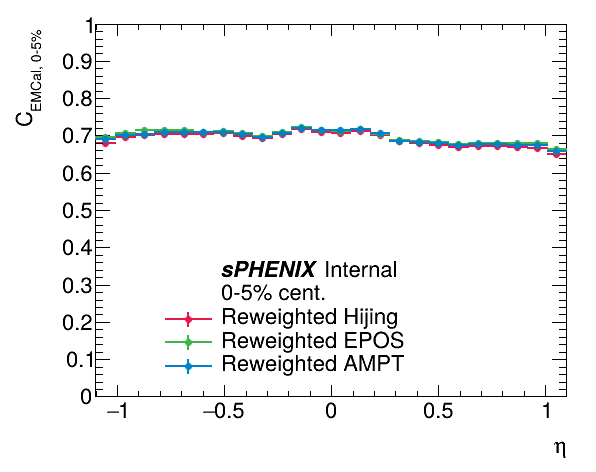
\includegraphics[width=0.48\linewidth]{detdeta/Figures/dETdeta_measurements/emcal_correction_factor_0-5.png}
    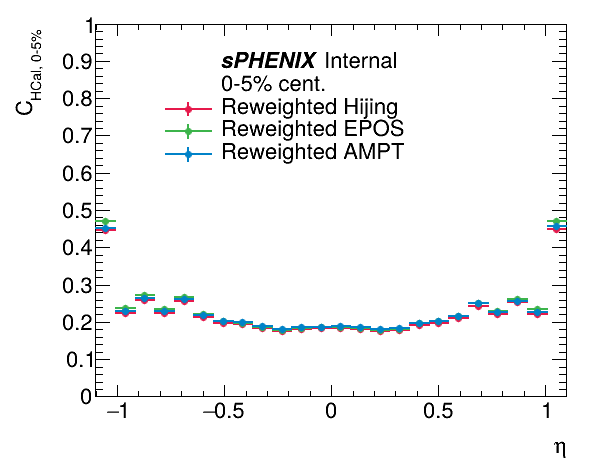
\includegraphics[width=0.48\linewidth]{detdeta/Figures/dETdeta_measurements/hcal_correction_factor_0-5.png}
    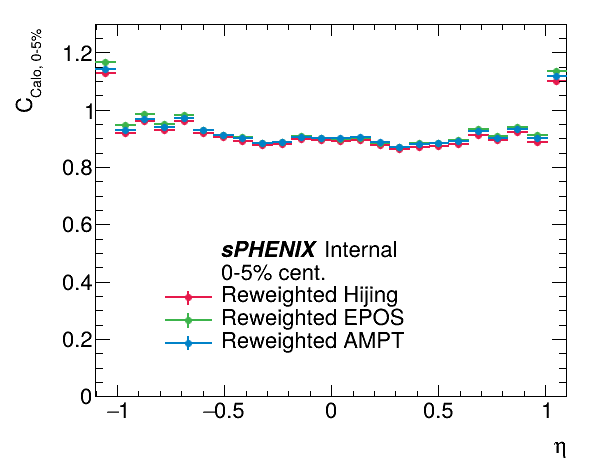
\includegraphics[width=0.48\linewidth]{detdeta/Figures/dETdeta_measurements/calo_correction_factor_0-5.png}
    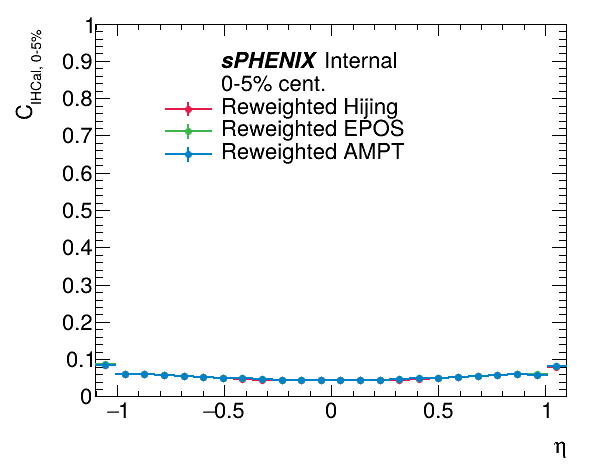
\includegraphics[width=0.48\linewidth]{detdeta/Figures/dETdeta_measurements/ihcal_correction_factor_0-5.png}
    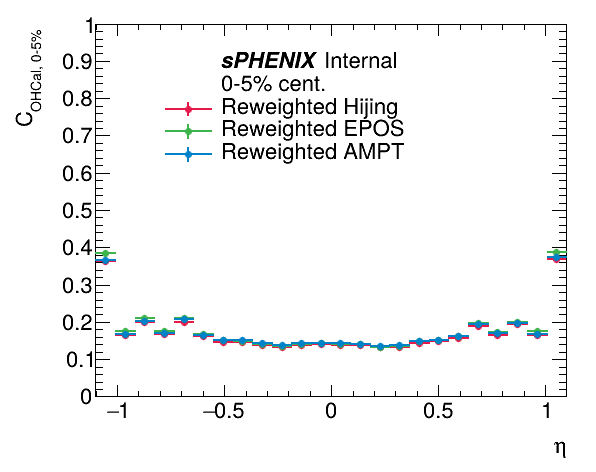
\includegraphics[width=0.48\linewidth]{detdeta/Figures/dETdeta_measurements/ohcal_correction_factor_0-5.png}
    \caption{Correction factors for 0-5\% central events for EMCal (upper left), HCal (upper right) and Full Calorimeter (middle left) as well as IHCal-only (middle right) and OHCal-only (lower) data. Correction factors calculated using reweighted HIJING, EPOS and AMPT MC datasets. Bad tower mask applied to correction factors to match tower acceptance in data.}
    \label{fig:correction_factors}
\end{figure}

\subsection{Effect of MC Reweighting on Correction Factors}

\subsection{Corrected \detdeta}
To obtain a fully corrected \detdeta, the truth \detdeta histogram is multiplied by the reconstructed \detdeta histogram from data, and divided by the reconstructed \detdeta histogram from simulation. 
In this way, there is compensation for non-uniform acceptance in the real detector by means of dividing out the reconstructed simulated \detdeta which has been artificially induced to have the same acceptance as reconstructed data \detdeta.

\begin{equation}
    \frac{\text{d}\ET}{\text{d}\eta}( \eta) = \frac{ \sum E_{\text{T,tower}}(\eta)}{C(\eta)}
\end{equation}

\subsection{Closure Test with MC Correction Factors}
Our application of \detdeta correction factors from MC datasets, EPOS, AMPT and HIJING, is validated using a half closure test for each of the three generator datasets for all calorimeter measurements and centrality bins presented in the \detdeta measurement. 

\begin{figure}
    \centering
    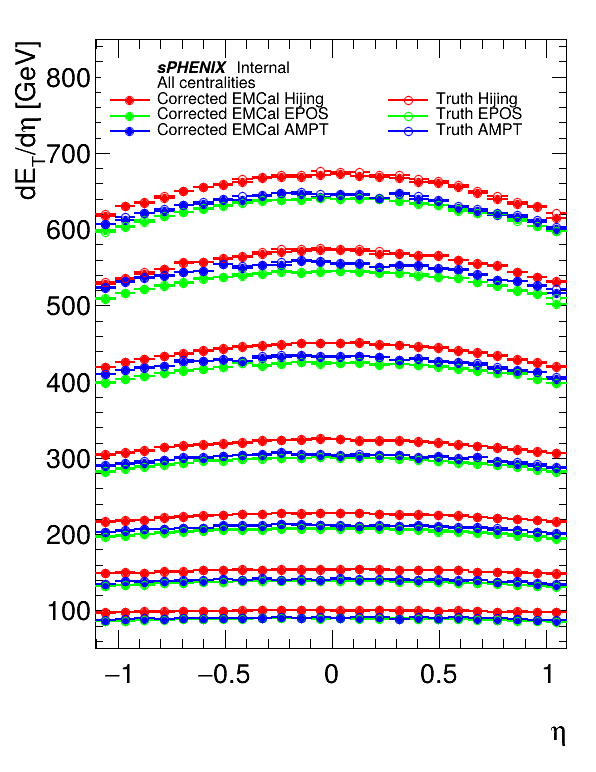
\includegraphics[width=0.48\linewidth]{detdeta/Figures/mc_closure/emcal_closure.png}
    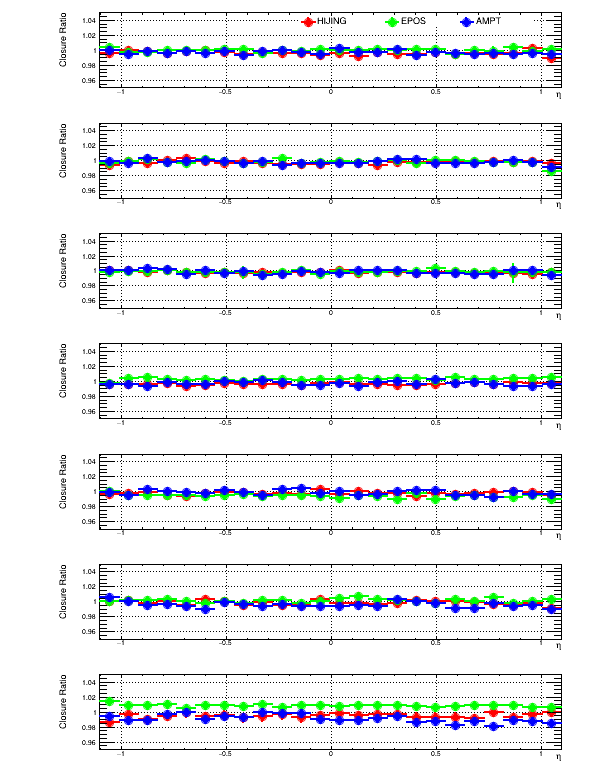
\includegraphics[width=0.48\linewidth]{detdeta/Figures/mc_closure/emcal_closure_ratio.png}
    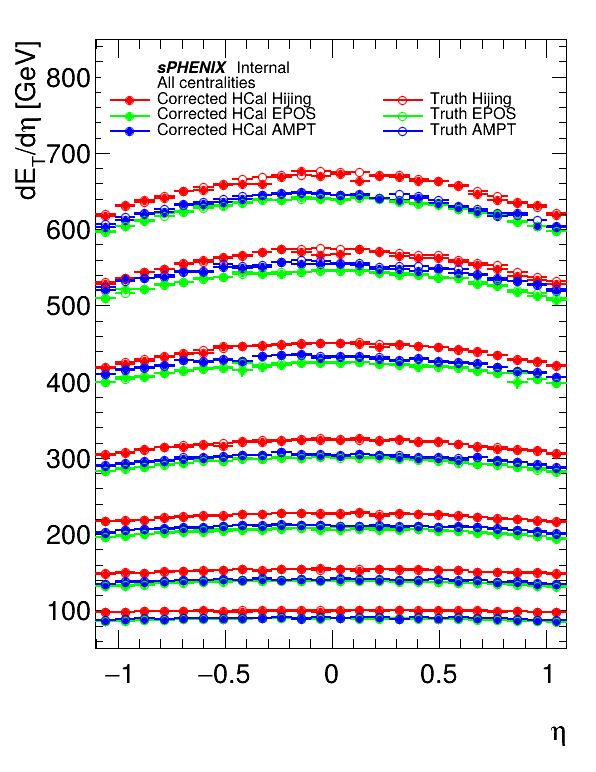
\includegraphics[width=0.48\linewidth]{detdeta/Figures/mc_closure/hcal_closure.png}
    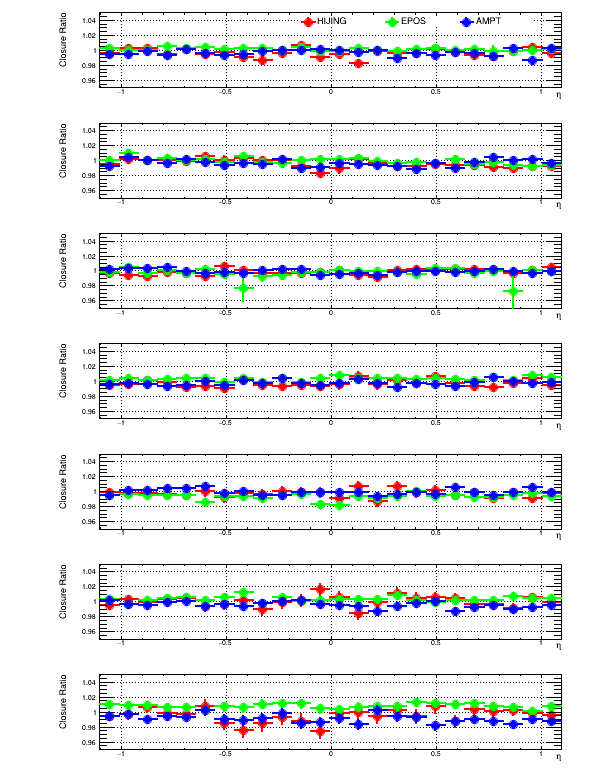
\includegraphics[width=0.48\linewidth]{detdeta/Figures/mc_closure/hcal_closure_ratio.png}
    \caption{Overlaid fully corrected and truth-level \detdeta for EMCal (top) and HCal (bottom) measurements (left plots). Ratio of fully corrected and truth-level \detdeta shown for each centrality bin (right plots).}
    \label{fig:emcal_hcal_closure}
\end{figure}

\begin{figure}
    \centering
    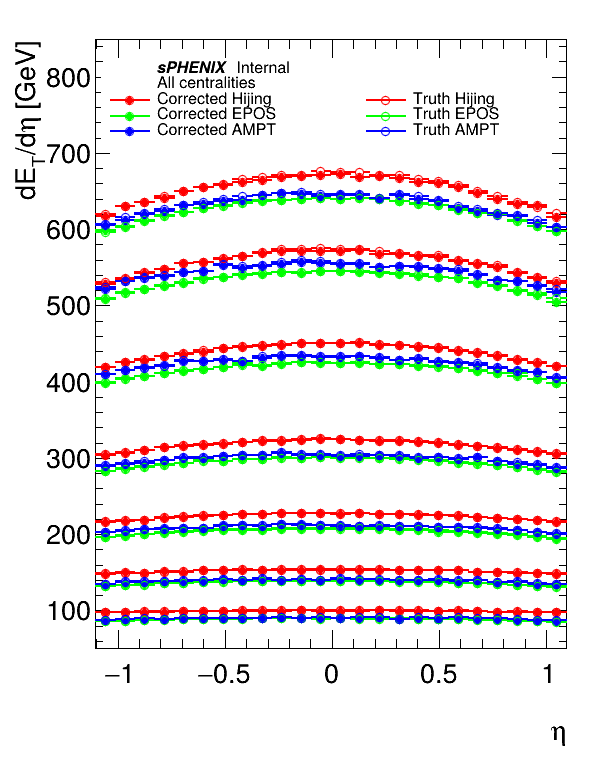
\includegraphics[width=0.48\linewidth]{detdeta/Figures/mc_closure/calo_closure.png}
    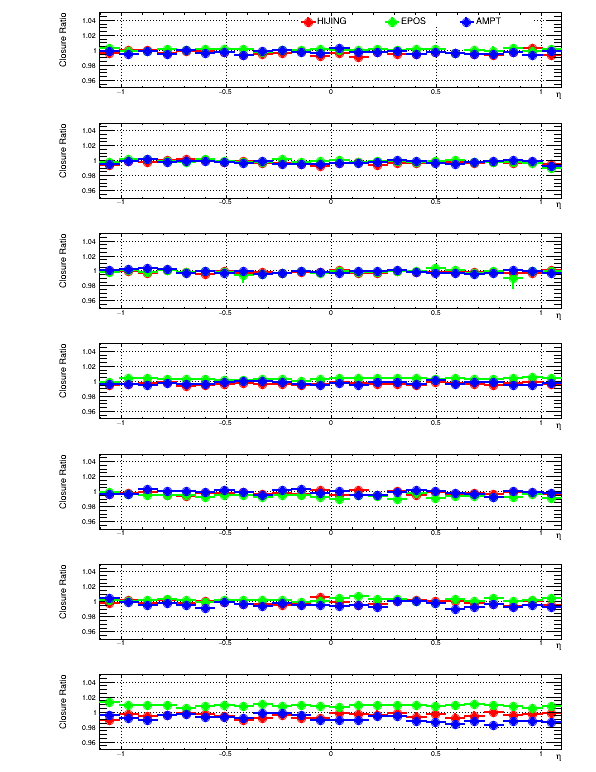
\includegraphics[width=0.48\linewidth]{detdeta/Figures/mc_closure/calo_closure_ratio.png}
    \caption{Overlaid fully corrected and truth-level \detdeta for Full Calorimeter measurements (left plots). Ratio of fully corrected and truth-level \detdeta shown for each centrality bin (right plots).}
    \label{fig:calo_closure}
\end{figure}